O principal desafio do sistema aéreo é manter a payload estável e em uma altitude constante. A câmera deve ser capaz de conseguir identificar a situação de risco sem que ocorra prejuízos nas imagens devido a má alocação do balão ou instabilidade do mesmo.

Para a flutuação será utilizado o princípio de Arquimedes do empuxo. Para fazer o balão flutuar, a força de empuxo deve ser maior que o peso total de toda a estrutura, portanto deve-se escolher os materiais mais leves e resistentes disponíveis no mercado.

Cada balão terá três pontos de fixação, esses pontos se encontram no teto dos prédios da universidade, porém alguns balões necessitarão de postes de fixação ao lado dos prédios. Cada balão terá dois pontos de fixação motorizados para que se possa realizar manutenções, os cabos e as junções devem suportar as tensões envolvidas no processo. Os cabos também devem ser dimensionados para suportar variações na velocidade do vento, que geram força de arrasto.
A seguir serão apresentadas mais detalhadamente  discussões e resultados referentes às questões levantadas acima.

\subsection{O Envelope} % (fold)
\label{sub:o_envelope}

\subsubsection{Gás do Balão}

	Existem duas possibilidades para a escolha do gás do balão cativo, o gás hélio e o gás hidrogênio. A seguir são apresentadas duas tabelas contendo as características físicas dos gases que podem ser escolhidos para o balão. Nas tabelas \ref{tab:caracHelio} e \ref{tab:caracHidro} as características do hélio e do hidrogênio são tiradas da empresa \textit{Gama Gases}.

	\begin{table}[H]
		\centering
		\caption[Características do Hélio]{Características do Hélio\cite{gamagases1}}
		\begin{tabular}{|c|c|}
			\hline
			\rowcolor[HTML]{FFFFFF}
			{\color[HTML]{000000} \textbf{Propriedades}}          & {\color[HTML]{000000} \textbf{Valores Numéricos}}   \\ \hline
			Densidade absoluta, gás a 101.325kPa a 0 ºC           & 0.1785 $Kg/m^3$                                     \\ \hline
			Densidade crítica                                     & 0.5307 $Kg/m^3$                                     \\ \hline
			Densidade relativa, gás a 101.325 kPa a 0 ºC, (ar = 1)& 0.138                                               \\ \hline
			Fator crítico de compressibilidade                    & 0.305                                               \\ \hline
			Fórmula                                               & 4He                                                 \\ \hline
			Massa Molecular                                       & 4.002602                                            \\ \hline
			Pressão crítica                                       & \begin{tabular}[c]{@{}c@{}}229 kPa ; 2.29 bar; 33.2 \\
			psia; 2.261 atm.\end{tabular}                                                                               \\ \hline
			Viscosidade, gás a 101.325 kPa a 26.8 ºC.             & 0.02012 mPa x s; 0.02012 cP.                        \\ \hline
			Volume específico a 21.1 ºC 101.325 kPa               & 6030.4$dm^3$/ kg; 96.6 $ft^3$/ Ib                   \\ \hline
		\end{tabular}
		\label{tab:caracHelio}
	\end{table}


\begin{table}[H]
	\centering
	\caption[Características do Hidrogênio]{Características do Hidrogênio~\cite{gamagases2}}
	\begin{tabular}{|c|c|}
		\hline
		\rowcolor[HTML]{FFFFFF}
		{\color[HTML]{000000} \textbf{Propriedades}}          & {\color[HTML]{000000} \textbf{Valores Numéricos}} \\ \hline
		Densidade absoluta, gás a 101.325kPa a 0ºC            & 0.08235 $Kg/m^3$                                  \\ \hline
		Densidade crítica                                     & 0.0310 $Kg/m^3$                                   \\ \hline
		Densidade relativa, gás a 101.325 kPa a 0ºC, (ar = 1) & 0.0695                                            \\ \hline
		Fator crítico de compressibilidade                    & 0.305                                             \\ \hline
		Fórmula                                               & H2                                                \\ \hline
		Limites de inflamabilidade no ar.                     & 4.0 à 75\% (por volume).                          \\ \hline
		Massa Molecular                                       & 2,01588                                           \\ \hline
		Pressão crítica                                       & \begin{tabular}[c]{@{}c@{}}1297 kPa; 12.97 bar; 188.1 psia;
	                                                                                                            \\
		12.80 atm.\end{tabular}                                                                                   \\ \hline
		Temperatura de auto-ignição.                          & \begin{tabular}[c]{@{}c@{}}844.3 K; 571.2 ºC;     \\
		1060 ºF.\end{tabular}                                                                                     \\ \hline
		Volume específico a 21.1 ºC, 101.325kPa.         			& 11967,4$dm^3$/kg; 191,7$ft^3$/lb.                 \\ \hline
	\end{tabular}
	\label{tab:caracHidro}
\end{table}

	O gás hidrogênio a primeira vista é mais vantajoso pois é mais leve que o hélio, sua densidade relativa ao ar é de 0.0695 enquanto que a do hélio é de 0.138, e apresentam um fator crítico de compressibilidade iguais. Porém o hidrogênio possui a característica de ser inflamável, enquanto que o hélio é conhecido por ser um gás inerte. Tendo em vista a segurança dos usuários do estacionamento e dos funcionários responsáveis pela manutenção do balão, a exposição ao sol e a possíveis, porém improváveis,  descargas elétricas o hélio se mostra a opção mais vantajosa.

	\subsubsection{Material do Envelope}

	Segundo \citeauthoronline{yajima} (\citeyear{yajima}), a maioria dos balões atmosféricos são feitos de filme de polietileno. A espessura dos envelopes dos balões usados pela NASA variam de 7 a 90 micrometros dependendo da altitude, funcionalidade, tempo de atividade e peso da payload e etc. Desta forma, cabe analisar que tipo de polietileno será utilizado para a confecção do envelope.

	Duas opções de polietileno foram analisadas, o Polietileno Linear de Baixa Densidade (PELBD) e o Polietileno de Baixa Densidade (PEBD). De acordo com \citeauthoronline{coutinho} (\citeyear{coutinho}), a temperatura máxima de atuação do PELBD é cerca de 120 ºC, sua massa específica varia numa faixa de 0.92 a 094 $g/cm^3$ e possui uma resistência à tração de 37 Mpa.

	A outra opção, o PEBD, segundo \citeauthoronline{coutinho} (\citeyear{coutinho}), trabalha a uma temperatura máxima de 110 ºC, possui uma massa específica de 0.92 $g/cm^3$ e resistência à tração de 24 Mpa.

	Outro material pesquisado foi o PVC pneumático, que possui densidade de 1.39 $g/cm^3$ \cite{innovainstrucao} e resistência a tração de 40 MPa E trabalha a uma temperatura máxima de 140 $^{\circ}$C \cite{datasheetPvc}. A tabela \ref{tab:tabmaterial} mostra os valores importantes dos materiais aqui citados.

	\begin{table}[htp]
		\centering
		\caption{Características dos materiais}
		\label{tab:tabmaterial}
		\begin{tabular}{ | c | c | c | c |}
			\hline
			\textbf{Material} &\textbf{Densidade} &\textbf{Resistência à tração} &\textbf{Temp. máx. de atuação}\\ \hline
			PELBD & 0.92 a 094 $g/cm^3$ &   37 MPa.&  120 $^{\circ}$C \\ \hline
			PEBD & 0.92 $g/cm^3$ &  24 MPa.&  110 $^{\circ}$C \\ \hline
			PVC & 1.39 $g/cm^3$ &  40 MPa.& 140 $^{\circ}$C \\
			\hline
		\end{tabular}
	\end{table}

	Analisando as duas opções de polietileno, o PELBD é o material mais adequado ao envelope do balão, pois possui melhor resistência mecânica e é leve, portanto, a priori ele seria o material escolhido, mas não foi possível encontra-lo na pesquisa de mercado, desta forma o material utilizado será o PVC pneumático.

% subsection o_envelope (end)

\subsection{Modelo do Balão} % (fold)
\label{sub:modelo_do_bal_o}

\subsubsection{Formato do Balão}
	De acordo com \citeauthoronline{yajima} (\citeyear{yajima}), existem vários formatos para balões atmosféricos, como o balão esférico, balão cilíndrico, balão tetraédrico e balão formato natural. O sistema mais fácil de ser trabalhado é o balão esférico, pois os cálculos de empuxo, volume, gás  apresentam menos complicações. Uma outra característica dos balões esféricos é a possibilidade do uso de uma fita de carga para suspender a payload no equador do envelope, o uso desse artifício tem por objetivo distribuir melhor a tensão na superfície do envelope.

	O esquema do balão pode ser observado na imagem \ref{img:balaoEsferico}.

	\begin{figure}[H]
		\centering
		\caption{Esquema de Balão Esférico com Fita de Carga.}
		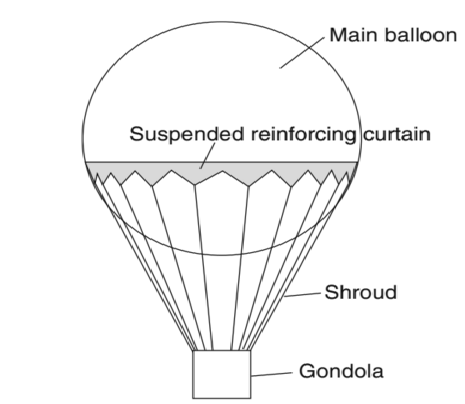
\includegraphics[width=0.5\textwidth]{figuras/balaoEsferico}
		\label{img:balaoEsferico}
	\end{figure}

	A fórmula para cálculo da tensão é a seguinte:

	\begin{equacao}
	\caption{Tensão do balão}
		\begin{equation}
			T = \frac{pr}{2}
		\end{equation}
		\label{eqn:calculoTensao}
	\end{equacao}

	Em que:
	\begin{description}
		\item[T] = tensão
		\item[p] = pressão interna do balão
		\item[r] = raio do balão
	\end{description}

\subsubsection{Sistema do Balão}

	Existem dois modelos de balões metereológicos empregados atualmente pela Agência Espacial Ameriacana (NASA), o sistema Zero Pressão (ZP) e o Super-Pressão (SP).

	O sistema ZP recebe esse nome porque a pressão interna do balão é a mesma  pressão do ambiente de atuação do sistema. Na parte de baixo do envelope do balão existe pelo menos um duto que permite a saída do gás dentro do balão para o alívio da pressão interna~\cite{nasa3}, como é exemplificado na figura \ref{img:maiorBalaoZeroPressao}.

	\begin{figure}[htp]
		\centering
		\caption[Maior Balão Zero Pressão Usado pela NASA]{Maior Balão Zero Pressão Usado pela NASA~\cite{nasa1}}
		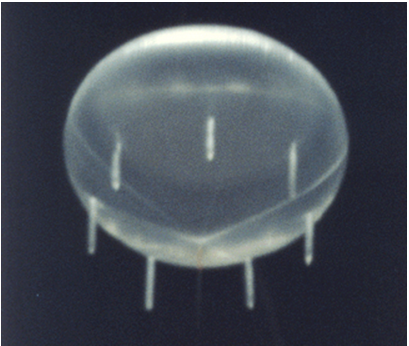
\includegraphics[width=0.5\textwidth]{figuras/maiorBalaoZeroPressao}
		\label{img:maiorBalaoZeroPressao}
	\end{figure}

	Para esse sistema normalmente é utilizado um material com 20 micrometros de espessura para o envelope. O balão é inflado em terra e é solto na atmosfera até que a força de empuxo seja igual ao seu peso. O duto funciona de tal modo que quando a pressão interna na base do balão excede a pressão da atmosfera exterior, o duto é empurrado para fora e forma uma um cilindro que permite que parte do gás seja expelida. Quando a diferença de pressão é negativa, a pressão atmosférica empurra o duto para dentro, impedindo a entrada de ar. Com a queda de temperatura, o gás esfria e contrai-se, diminuindo o volume e consequentemente o empuxo. Em balões atmosféricos usado pela NASA, para manter a altitude constante durante a noite o balão solta pesos c, como por exemplo areia, durante esse período a quantidade de gás dentro do envelope é a mesma pois o duto se fecha quando o gás se contrai~\cite{eoss}. Porém, no próximo dia, com o aumento da temperatura o gás irá se expandir, aumentando o volume e subindo mais, pois estará mais leve. Para manter uma altitude a mais constante possível, segundo a \citeauthoronline{nasa3} (\citeyear{nasa3}), um balão desse tipo requer uma perda de 6 a 8\% de massa quando a temperatura diminui. O principal problema desse tipo de sistema é a perda de gás pelo duto aberto ao ambiente.

	O sistema SP possui a vantagem de ser completamente vedado, ou seja, não perde gás durante seu período de atividade. Por esse fato o balão tem uma pressão interna maior que a pressão externa e isso implica no aumento da espessura do envelope, normalmente cerca de 10 vezes maior que a espessura de um balão ZP~\cite{yajima}. A figura \ref{img:distribuicaoPressao} mostra a distribuição de pressão de um balão atmosférico da NASA, percebe-se que o equador do envelope é a área de maior concentração de pressão, esse fato exige que a parte de fixação seja reforçada para que o envelope não seja danificado.

	\begin{figure}[htp]
		\centering
		\caption[Distribuição de Pressão de um Balão Super Pressão]{Distribuição de Pressão de um Balão Super Pressão~\cite{nasa2}}
		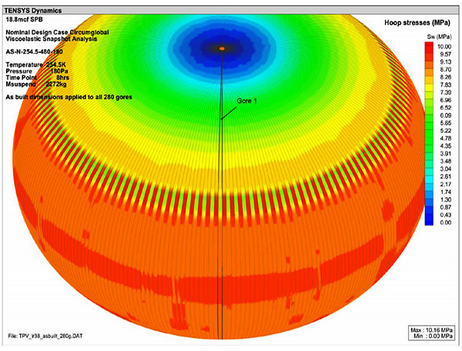
\includegraphics[width=0.5\textwidth]{figuras/distribuicaoPressao}
		\label{img:distribuicaoPressao}
	\end{figure}

	Em linhas gerais o balão ZP é mais leve, porém possui o problema de perder gás durante sua operação. O balão SP tem a vantagem de não perder gás durante sua operação, porém é mais pesado pois precisa ter um envelope mais grosso. Pelo fato de não haver saída de gás, visando economia de hélio durante a operação, o sistema escolhido será o sistema Super Pressão.



\subsection{Cálculo  do Volume do Balão} % (fold)
\label{sub:c_lculo_do_volume_do_bal_o}

	\subsubsection{Cálculo Preliminar do Volume do Balão}

	O diagrama de corpo livre do balão pode ser observado na imagem \ref{img:corpoLivreBalao}.
	\begin{figure}[H]
		\centering
		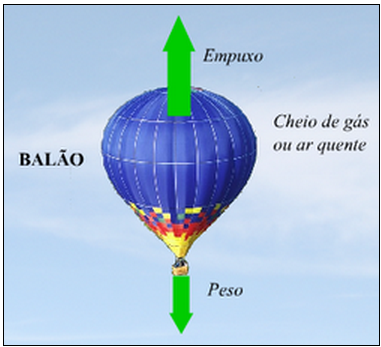
\includegraphics[width=0.5\textwidth]{figuras/corpoLivreBalao}
		\caption[Diagrama de Corpo Livre de um Balão]{Diagrama de Corpo Livre de um Balão~\cite{justino}}
		\label{img:corpoLivreBalao}
	\end{figure}

	O volume do balão foi calculado primeiramente desprezando a tensão e o peso dos cabos. 	O volume do gás Hélio foi calculado da seguinte maneira:

	Partindo do principio de que o volume de gás tem que gerar uma força de empuxo maior que a força peso, como mostrado na figura \ref{img:corpoLivreBalao}, para que o balão consiga ficar a uma certa altitude. Os cabos de apoio do balão foram desconsiderados nesse cálculo preliminar. A partir disso considerou-se a equação \eqref{eqn:calcEmpuxo} para o calculo de empuxo.

	\begin{equacao}
	\caption[Fórmula para o cálculo de empuxo]{Fórmula para o cálculo de empuxo~\cite[pp.~63--65]{munson}}
		\begin{equation}
			E = \rho_{ar} \cdot g \cdot V
		\end{equation}
		\label{eqn:calcEmpuxo}
	\end{equacao}

	Em que:
	\begin{description}
		\item[$\boldsymbol{\rho_{ar}}$] = massa especıfica do ar
		\item[$\boldsymbol{g}$] = aceleração da gravidade
		\item[$\boldsymbol{V}$] = volume do fluído deslocado
	\end{description}

	A massa de helio ($M_{h}$) é calculada segundo a equação \eqref{eqn:calcMassaHelio}.

	\begin{equacao}
	\caption{Fórmula para o cálculo da massa do hélio}
		\begin{equation}
			M_{h} = 0.138 \cdot \rho_{ar} \cdot g \cdot V
		\end{equation}
		\label{eqn:calcMassaHelio}
	\end{equacao}

	A massa de material foi calcula pela equação \eqref{eqn:calcMassaMaterial}.

	\begin{equacao}
	\caption{Fórmula para o cálculo da massa do material}
		\begin{equation}
			M_{h} = \rho_{m} \cdot e_{m} \cdot A
		\end{equation}
		\label{eqn:calcMassaMaterial}
	\end{equacao}

	Em que:
	\begin{description}
		\item[$\boldsymbol{A}$] = área do envelope
		\item[$\boldsymbol{\rho_{m}}$] = massa expecífica do material ($940Kg/m^3$)
		\item[$\boldsymbol{e_{m}}$] = espessura do material ($20mu m$)
	\end{description}

	A massa da \emph{payload} foi estimada em cerca de 5kg, e para margem de segurança, os cálculos foram realizados com uma massa de 10kg. A equação \eqref{eqn:calcBalancoForca} foi utilizada para realizar o cálculo do balanço das forças.

	\begin{equacao}
	\caption{Fórmula para o cálculo do balanço das forças}
		\begin{equation}
			E = g \cdot (M_{h} + M_{p} + M_{m})
		\end{equation}
		\label{eqn:calcBalancoForca}
	\end{equacao}

	Substituindo \eqref{eqn:calcEmpuxo}, \eqref{eqn:calcMassaHelio}, \eqref{eqn:calcMassaMaterial} em \eqref{eqn:calcBalancoForca}, temos a equação \eqref{eqn:eqResultante1}.

	\begin{equacao}
	\caption{Equação resultante de \eqref{eqn:calcEmpuxo}, \eqref{eqn:calcMassaHelio} e \eqref{eqn:calcMassaMaterial}}
		\begin{equation}
			\rho_{ar} \cdot g \cdot V = g(M_{h} + M_{p} + M_{m})
		\end{equation}
		\label{eqn:eqResultante1}
	\end{equacao}

	Como trata-se de um balão esférico temos que $V = \frac{1}{3} \cdot 4 \pi \cdot r^2$. Voltando a equação \eqref{eqn:eqResultante1}, isolando e agrupando os termos semelhantes temos:

	\begin{equacao}
	\caption{Equação resultante de \eqref{eqn:eqResultante1}}
		\begin{equation}
			\frac{1}{3} \cdot \rho \cdot 4 \pi \cdot r^3 \cdot (1 - 0.138) - 18.8 \cdot 10^{-3} \cdot 4 \pi \cdot r^2 - 10 = 0
		\end{equation}
		\label{eqn:eqResultante2}
	\end{equacao}

	Substituindo os valores e usando o metodo de Newton~\cite[pp.~174--175]{hoffman} para calcular as raızes de polinômios para resolver a equação \eqref{eqn:eqResultante2}, foi encontrado um valor para o raio de 1.4 metros. Logo o balao teria que ter pelo menos 1.4 metros de raio. A partir desse valor calcula-se o empuxo, o peso do helio, o peso e a quantidade de polietileno que o balao ira precisar. Para o cálculo do empuxo considerou-se ar  = $1.11166 kg/m^3$, que é a densidade do ar a 1000m de altitude. Considerou-se h = 0.138 ar que é a massa específica do hélio. A tabela \ref{tab:forcasVerticaisAtuantes} mostra todos os valores de forças verticais atuantes no balão.

	\begin{table}[htp]
		\centering
		\caption{Forças Verticais Atuantes no Balão}
		\begin{tabular}{|c|c|}
			\hline
			\rowcolor[HTML]{FFFFFF}
			{\color[HTML]{000000} \textbf{Grandezas}} & {\color[HTML]{000000} \textbf{Valores Numéricos (N)}} \\ \hline
			Empuxo                                    & 138.1                                                 \\ \hline
			Peso do Hélio                             & 19.1                                                  \\ \hline
			Peso do material do envelope              & 4.6                                                   \\ \hline
			Peso da Payload                           & 100                                                   \\ \hline
		\end{tabular}
		\label{tab:forcasVerticaisAtuantes}
	\end{table}

	As contas acima foram realizadas para que se tivesse uma ideia inicial do tamanho do balão e da ordem de grandeza das forças associadas.

\subsubsection{Cálculo Real do Volume do Balão}

O  balão irá operar em uma faixa de altura entre 20 e 25 metros em relação ao solo, porém  o mesmo será fixado no alto dos prédios da Universidade de Brasília no Campus do Gama, esses prédios têm uma altura de 10 a 12 metros dependendo do prédio. Desta forma, foram decididos os pontos de fixação e calculado o tamanho dos cabos, e concluiu-se que os cabos deveriam ter no máximo 20 metros de comprimento.

O cabo de aço escolhido tem um diâmetro de 6,4 mm e tem massa aproximada de 146 gramas por metro, um balão precisa de três cabos de sustentação de 20 metros cada. Desta forma o peso devido a massa dos cabos está descrito na equação \eqref{eqn:pesoCabos}.

\begin{equacao}
\caption{Peso dos cabos}
	\begin{equation}
		P_{c} = C \cdot m \cdot g \cdot n_{c} \implies 20 \cdot 0.146 \cdot 9,8 \cdot 3 = 86 N
	\end{equation}
	\label{eqn:pesoCabos}
\end{equacao}

Em que:
\begin{description}
	\item[$\boldsymbol{P_{c}}$] = peso dos cabos
	\item[$\boldsymbol{C}$] = comprimento do cabo
	\item[$\boldsymbol{m}$] = massa por unidade de comprimento
	\item[$\boldsymbol{g}$] = aceleração da gravidade
	\item[$\boldsymbol{n_{c}}$] = número de cabos
\end{description}

O cabo de alimentação energética tem uma massa aproximada de 50 gramas por metro, como esse cabo não pode sofrer esforço mecânico, ele nunca  ficará tensionado e para isso seu comprimento deverá ser maior que o comprimento dos outros cabos. Para o cálculo do peso desse cabo seu comprimento será de 25 metros, procedendo da mesma forma no cálculo dos outros cabos temos: $25 \cdot 0.05 \cdot 9.8 = 13 N$. Portanto o peso total dos cabos será na faixa de 100 N.

Ainda existem peças que não foram levadas em consideração nessa conta como os mosquetões, sistema de estabilização entre outros. Admiti-se que essa carga extra não ultrapasse o valor de 20 N. Por margem de segurança usaremos um envelope com 60 micrometros de espessura.

A tabela \ref{tab:forcasAtuantes} mostra todos os valores de forças verticais atuantes no balão. Para o cálculo do empuxo considerou-se $\rho_{ar}$ = $1.11166 kg/m^3$, que é a densidade do ar a 1000m de altitude. Considerou-se $\rho_{h} = 0.138 \rho_{ar}$, que é a massa específica do hélio. A tabela \ref{tab:forcasAtuantes} apresenta todas as forças atuantes no balão.

\begin{table}[htp]
	\centering
	\caption[Forças Atuantes no Balão]{Forças Atuantes no Balão. Volume de $113.1 m^2$}
	\begin{tabular}{|c|c|}
		\hline
		\rowcolor[HTML]{FFFFFF}
		{\color[HTML]{000000} \textbf{Forças}} & {\color[HTML]{000000} \textbf{Valores Numéricos (N)}} \\ \hline
		Empuxo                                 & 1232.1                                                \\ \hline
		Peso do Hélio                          & 170                                                   \\ \hline
		Peso do material do envelope           & 62.5                                                  \\ \hline
		Peso dos Cabos                         & 100                                                   \\ \hline
		Peso Extra                             & 20                                                    \\ \hline
		Peso da Payload                        & 100                                                   \\ \hline
		Empuxo Líquido                         & 780                                                   \\ \hline
	\end{tabular}
	\label{tab:forcasAtuantes}
\end{table}


\subsection{Forças no Balão} % (fold)
\label{sub:for_as_no_bal_o}

De acordo com \citeauthoronline{yajima} (\citeyear{yajima}), a força \textbf{F} que atua no balão devido ao vento relativo tem duas componentes: A força de arrasto, que atua paralelamente a direção do vento relativo, e a força lateral, que atua perpendicular à direção do vento.

Tais forças são descritas pelas equações \eqref{eqn:forcaArrasto} \eqref{eqn:forcaLateral}.

	\begin{equacao}
	\caption[Força de arrasto]{Força de Arrasto~\cite{yajima}}
		\begin{equation}
			F_{d} = \frac{1}{2} \rho_{ar} \left | v_{w} - v_{b} \right |^{2} C_{d}A{b}
		\end{equation}
		\label{eqn:forcaArrasto}
	\end{equacao}

	\begin{equacao}
	\caption[Força lateral]{Força Lateral~\cite{yajima}}
		\begin{equation}
			F_{y} = \frac{1}{2} \rho_{ar} \left | v_{w} - v_{b} \right |^{2} C_{y}A{b}
		\end{equation}
		\label{eqn:forcaLateral}
	\end{equacao}

	Em que:
	\begin{description}
		\item[$\boldsymbol{F_{d}}$] = Força de Arrasto;
		\item[$\boldsymbol{F_{y}}$] = Força Lateral;
		\item[$\boldsymbol{\rho_{a}}$] = Densidade do Ar;
		\item[$\boldsymbol{C_{d}}$] = Coeficiente de Arrasto;
		\item[$\boldsymbol{C_{y}}$] = coeficiente de força lateral efetiva;
		\item[$\boldsymbol{A_{b}}$] = Area Frontal.
	\end{description}

	Considerando que o balão de monitoramento deve permanecer parado, podemos considerar que a velocidade do balão é nula, e a força de arrasto e força lateral se darão apenas em função da velocidade do vento.

	Para o calcula da força de arrasto e força lateral então é necessário conhecer a velocidade do vento que incidirá sobre o balão. Para determinar a velocidade do vento entramos no Banco de Dados Histórico do Instituto Nacional de Meteorologia~\cite{inmet}. Para termos um valor que nos desse uma margem de segurança analisamos os dados de 01/01/2005 a 01/01/2015. No período avaliado a maior velocidade do vento ocorrida no DF registrada foi de 17 m/s.

	O Coeficiente de Arrasto e o coeficiente de força lateral está diretamente relacionado ao número de Reynolds. O número de Reynolds é um número adimensional usado em mecânica dos fluidos para o cálculo do regime de escoamento de determinado fluido dentro de um tubo ou sobre uma superfície.~\cite{bird}. Segundo \citeauthoronline{yajima} (\citeyear{yajima}), o número de Reynolds para um balão é dado pela equação \eqref{eqn:numeroReynolds}.

	\begin{equacao}
	\caption{Número de Reynolds para balão}
		\begin{equation}
			Re_{b} = \frac{\rho_{ar} D_{b} \mid V_{w} - V_{b} \mid}{\mu_{a}}
		\end{equation}
		\label{eqn:numeroReynolds}
	\end{equacao}

	Em que:
	\begin{description}
		\item[$\boldsymbol{Re_{b}}$] = Número de Reynolds;
		\item[$\boldsymbol{D_{b}}$] = Diâmetro do Balão;
		\item[$\boldsymbol{V_{w}}$] = Velocidade do Vento;
		\item[$\boldsymbol{V_{b}}$] = Velocidade do Balão;
		\item[$\boldsymbol{\mu_{a}}$] = coeficiente de viscosidade do Ar .
	\end{description}

	Considerando que o balão terá um diâmetro de 6m e a Brasília se encontra a uma altitude próxima a 1000m acima do nível do Mar. Temos que:

	\begin{description}
		\item[Densidade do Ar a 1km de altitude:] $\rho_{a}$ = $1,11166 Kg/m^3$ segundo a tabela de atmosfera padrão~\cite{bird};
		\item[Diâmetro do Balão:] 6m;
		\item[Velocidade máxima do vento observada:] 17 m/s;
		\item[Viscosidade do Ar:] 0.01813 mPa.s~\cite{bird}.
	\end{description}

	Logo, obtemos a equação \eqref{eqn:numeroReynoldsBalai}.

	\begin{equacao}
	\caption{Número de Reynolds para balão}
		\begin{equation}
			Re_{e} = \frac{1.11166 kg/m^3 \cdot 6m \cdot 17 m/s}{0.01813 \cdot 10^{-3} Pa.s} \implies Re_{b} = 6.354 \cdot 10^6
		\end{equation}
		\label{eqn:numeroReynoldsBalai}
	\end{equacao}

	A figura \ref{img:coeficienteArrasto} mostra o coeficiente de arrasto do balão em função do número de Reynolds do fluido e do formato do balão. Para o número de Reynolds da ordem de 6 x 106  temos um coeficiente de arrasto de aproximadamente 0.2.

	\begin{figure}[htp]
		\centering
		\caption[Coeficiente de arrasto do balão em função do número de Reynolds do fluido e do formato do balão]{Coeficiente de arrasto do balão em função do número de Reynolds~\cite{myers}}
		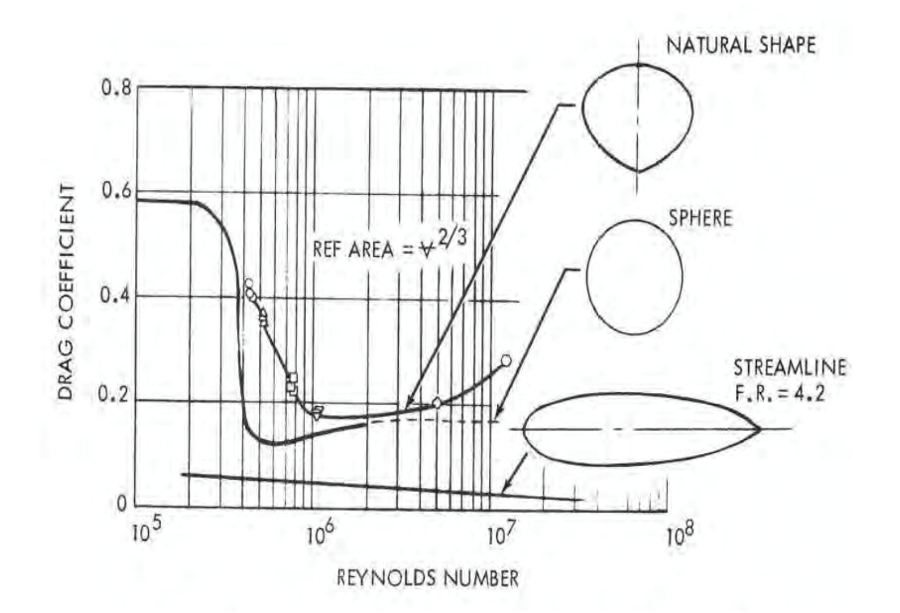
\includegraphics[width=0.5\textwidth]{figuras/coeficienteArrasto}
		\label{img:coeficienteArrasto}
	\end{figure}

	Tendo em mão esses valores podemos então calcular a força máxima de arrasto que o balão estará sujeito a partir da \eqref{eqn:forcaArrasto}, obtendo a equação \eqref{eqn:forcaArrastoMax}.

	\begin{equacao}[htp]
	\caption{Força máxima de arrasto que o balão estará sujeito}
		\begin{equation}
			F_{D} = \frac{1}{2} \cdot 1.11166 \frac{Kg}{m^{3}} \cdot \left | 17m/s \right |^{2} \cdot 0.2 \cdot 28.273m^{2} \implies F_{D} = 908.2 N
		\end{equation}
		\label{eqn:forcaArrastoMax}
	\end{equacao}

	O coeficiente de força lateral efetiva para um balão que se encontra estacionário é de 0.18~\cite{ferguson}. Podemos observar que nas duas equações este é o único valor que se altera, logo temos que:

	\begin{equacao}[htp]
	\caption{Força máxima lateral que o balão estará sujeito}
		\begin{equation}
			F_y = 817.38 N
		\end{equation}
		\label{eqn:forcaLateralMax}
	\end{equacao}

	Temos então que sobre o balão atuaram as seguintes forças:

	\begin{description}
		\item[Força de arrasto:] 908.2 N
		\item[Força lateral:] 817.38 N
		\item[Força de empuxo:] 800 N
	\end{description}

	O que dá origem a equação \eqref{eqn:forcaResultante}.

	\begin{equacao}
	\caption{Força resultante}
		\begin{equation}
			F_D = \sqrt{908.2^2 + 817.38^2 + 800^2} \implies F_D = 1460.458 N
		\end{equation}
		\label{eqn:forcaResultante}
	\end{equacao}

\subsection{Posicionamento dos cabos}

	A posição em relação ao balão a qual os cabos estarão fixados possui grande importância, pois o mal posicionamentos deles poderá levar o balão a uma condição de instabilidade, logo prejudicando o monitoramento. O balão será fixado por três cabos, cuja  configuração é mostrada pela figura \ref{img:coordcabos}.

	\begin{figure}[htp]
		\centering
		\caption[Coordenadas do cabo]{Coordenadas do cabo~\cite{beer}}
		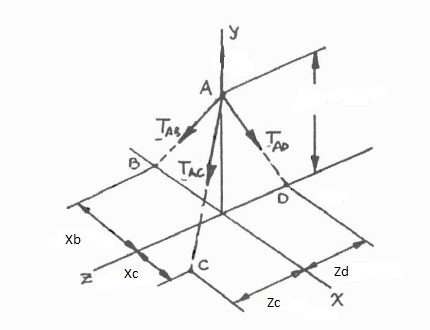
\includegraphics[width=0.8\textwidth]{figuras/coorcabo}
		\label{img:coordcabos}
	\end{figure}

	Serão utilizados cinco balões, que serão posicionados de acordo com a seguinte configuração: dois balões estarão em cima da Unidade de Ensino e Docência (UED) e outros dois balões no terraço na Unidade Acadêmica (UAC). Para estes balões, dois cabos estarão fixados no topo do prédio (pontos B e C na figura) e um terceiro cabo será preso numa haste (pontos C) de 10 m de altura que ficará a uma determinada distância dos prédios. O quinto balão ficará posicionado em cima do restaurante universitário (RU), onde dois cabos serão fixados em cima do RU (pontos B e D) e o terceiro cabo será preso a uma haste (ponto C) que possui a altura do restaurante universitário.

	Para que o balão fique em uma posição de equilíbrio o sistema de equações \eqref{eq:sustentacaoCabos}.

\begin{equacao}
	\caption{Sistema de sustentação dos cabos}
	\label{eq:sustentacaoCabos}
	\begin{equation}
		\begin{bmatrix}
			-\frac{X_b}{L_B}T_{AC} & -\frac{Y-Y_p}{L_B}T_{AB} & 0\\
			-\frac{X_c}{L_C}T_{AB} & -\frac{Y-Y_h}{L_C}T_{AC} & \frac{Z_c}{L_C}T_{AC}\\
			0 & -\frac{Y-Y_p}{L_D}T_{AD} & -\frac{Z_d}{L_D}T_{AD}
		\end{bmatrix}
		\begin{bmatrix}
			i\\
			j\\
			k
		\end{bmatrix}
		 =
		\begin{bmatrix}
			F_{dx}\\
			E_L\\
			F_{dz}
		\end{bmatrix}
	\end{equation}
\end{equacao}



	Em que:
	\begin{description}
		\item[$\boldsymbol{L_{B}}$] = Comprimento do cabo do ponto A até o ponto B
		\item[$\boldsymbol{L_{C}}$] = Comprimento do cabo do ponto A até o ponto C
		\item[$\boldsymbol{L_{D}}$] = Comprimento do cabo do ponto A até o ponto D
		\item[$\boldsymbol{E_{L}}$] = Empuxo líquido
		\item[$\boldsymbol{F_{D}}$] = Força de arrasto
		\item[$\boldsymbol{F_{dx}}$] = Componente - x da força aerodinâmica
		\item[$\boldsymbol{F_{dz}}$] = Componente - z da força aerodinâmica
		\item[$\boldsymbol{Y}$] = Altura do balão
		\item[$\boldsymbol{Y_{p}}$] = Altura do prédio
		\item[$\boldsymbol{Y_{h}}$] = Altura da haste
	\end{description}

A melhor abordagem para resolver este sistema é definir aonde estarão fixados os cabos ($x_{b}$, $x_{c}$, $z_{c}$, $z_{d}$) e estabelecer o comprimento de cada cabo ($L_{B}$, $L_{C}$, $L_{D}$), logo as incógnitas serão as forças em cada cabo ($T_{AB}$, $T_{AC}$, $T_{AD}$). Portanto, deve-se escolher as posições dos cabos que forneçam valores de forças fisicamente possíveis. Outro ponto importante é que a força do cabo que é fixado na haste seja bem inferior em relação as forças dos cabos preso aos prédios, logo será necessário o uso de uma haste com simples resistência a tração, ao invés de uma haste com boas propriedades mecânica no então de custo elevado. A disposição dos cabos pode ser observada na tabela \ref{tab:composangcabos}.

\begin{table}[htp]
\centering
\caption{Posição, comprimento e ângulo dos cabos}
\begin{tabular}{l|l|l|l|l|l|l|l|l|l|l|}
\cline{2-11}
 & $X_{b}$ m & $X_{c}$ m & $Z_{c}$ m & $Z_{d}$ m & $L_{b}$ m & $L_{c}$ m & $L_{D}$ m & $\Theta _{B}$ & $\Theta _{C}$ & $\Theta _{D}$ \\ \hline
\multicolumn{1}{|l|}{UED} & 18,0 & 5,0 & 10.0 & 18,0 & 23.5 & 18,7 & 23.5 & 39,8 & 45,0 & 39,8 \\ \hline
\multicolumn{1}{|l|}{UAC} & 18,0 & 5,0 & 10.0 & 18,0 & 23.5 & 18,7 & 23.5 & 39,8 & 45,0 & 39,8 \\ \hline
\multicolumn{1}{|l|}{RU} & 25,0 & 5,0 & 15,0 & 25,0 & 32,7 & 26,3 & 32,7 & 40.3 & 46,4 & 40.3 \\ \hline
\end{tabular}
\label{tab:composangcabos}
\end{table}

	Para as condições de projeto:

	O empuxo líquido, $E_{L}$, foi calculado anteriormente, o seu valor é de 800 N. A forca de arrasto, $F_{D}$ é de aproximadamente 880 N. Portando a força total exercida nos cabos é de aproximadamente 1200 N. Assume-se que a força de arrasto é dividida igualmente entre a componente x e z: $F_{dx}$ = 440 N e $F_{dz}$ = 440 N.

	\begin{itemize}
		\item Altura do balão = 10 m
 		\item Altura do UED = 10 m
 		\item Altura do UAC = 10 m
 		\item Altura do RU = 4 m
 		\item Altura da haste = 10 m
	\end{itemize}

Portanto, para os balões presentes no UED e UAC, o cabo fixado na haste ficará aproximadamente a 12 metros do prédio, e o cabos que estão presos no terraço estão a aproximadamente 18 metros do balão. Para o balão posicionado no RU, o cabo na haste estará a 16 metros do prédio, e os cabos fixados no topo do prédio a 25 metros do balão. As tensões presentes estão dispostas na tabela \ref{table:modTensoes}.

\begin{table}[htp]
\centering
\caption{ Módulo das tensões}
\begin{tabular}{l|l|l|l|}
\cline{2-4}
 & $T_{AB}$ [N] & $T_{AC}$ [N] & $T_{AD} [N]$ \\ \hline
\multicolumn{1}{|l|}{UED} & 588,53 & 45,35 & 604,31 \\ \hline
\multicolumn{1}{|l|}{UAC} & 588,53 & 45,35 & 604,31 \\ \hline
\multicolumn{1}{|l|}{RU} & 585,13 & 42,28 & 606,14 \\ \hline
\end{tabular}
\label{table:modTensoes}
\end{table}

A figura \ref{img:pos-bal} mostra como deve ser posicionado um dos balões, nota-se que dois pontos de sustentação estão no teto do prédio e o terceiro ponto é um poste. Os dois pontos em cima do prédio possuem motores para puxar o balão para baixo e controlar sua altitude.

\begin{figure}[htp]
	\centering
	\caption{Posicionamento de um dos balões}
	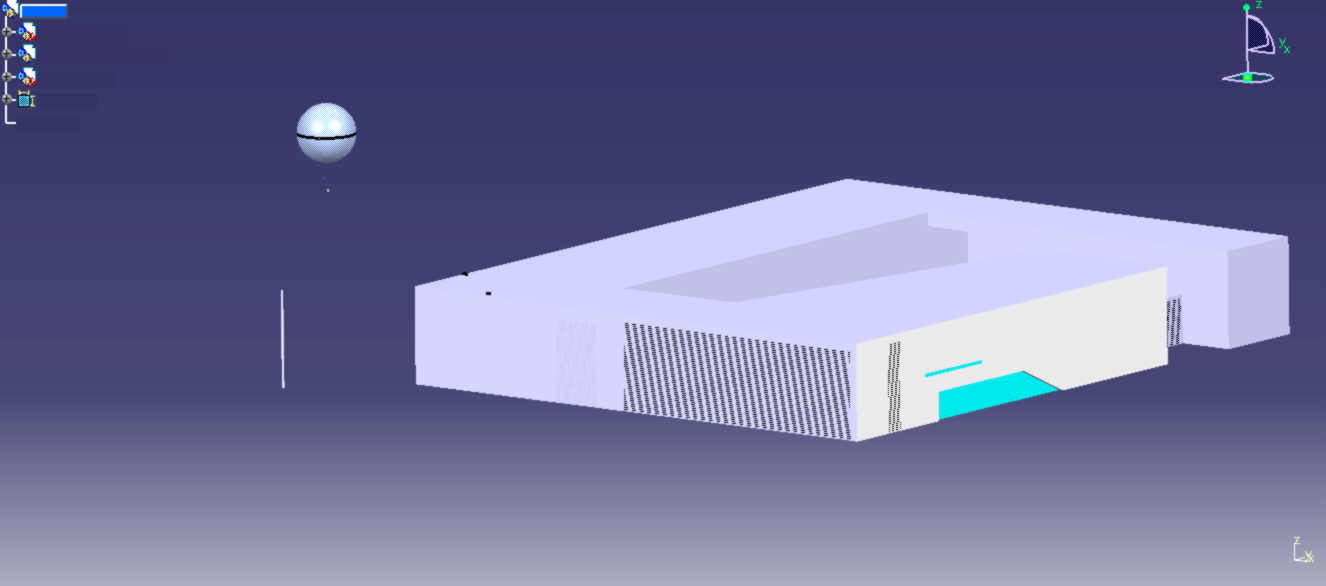
\includegraphics[width=0.8\textwidth]{figuras/pos-bal}
	\label{img:pos-bal}
\end{figure}

\subsection{Sustentação do SUM}

O Balão Cativo será fixado em três pontos diferentes (figura \ref{img:catiaPayload}) para que seja garantida sua estabilidade considerando ventos laterais de qualquer direção, adotou-se o modelo de balão de zero pressão de formato esférico preenchido com gás hélio. No caso dos balões de zero pressão há uma perda diária do volume de gás de cerca de 8\%. O volume de gás hélio no balão será de 113m$^{3}$ e, considerando as perdas diárias, estima-se que a cada sete dias haverá a necessidade de  efetuar uma reposição desse gás para garantir o bom funcionamento do monitoramento do estacionamento, onde o empuxo gerado pelo gás seja suficiente para manter uma altitude de 20m.

	Na figura \ref{img:catia1} está o protótipo do SUM. Nota-se que há uma fita de carga que passa no equador do envelope que segura a payload. A figura \ref{img:catiaPayload} mostra como a payload deve ser amarrada ao balão. A figura \ref{img:catia2} mostra o detalhe do trilho na parte superior da payload, com esse trilho a payload pode se mover sem que haja perda no foco da imagem.

	\begin{figure}[htp]
		\centering
		\caption{Protótipo do SUM no Catia.}
		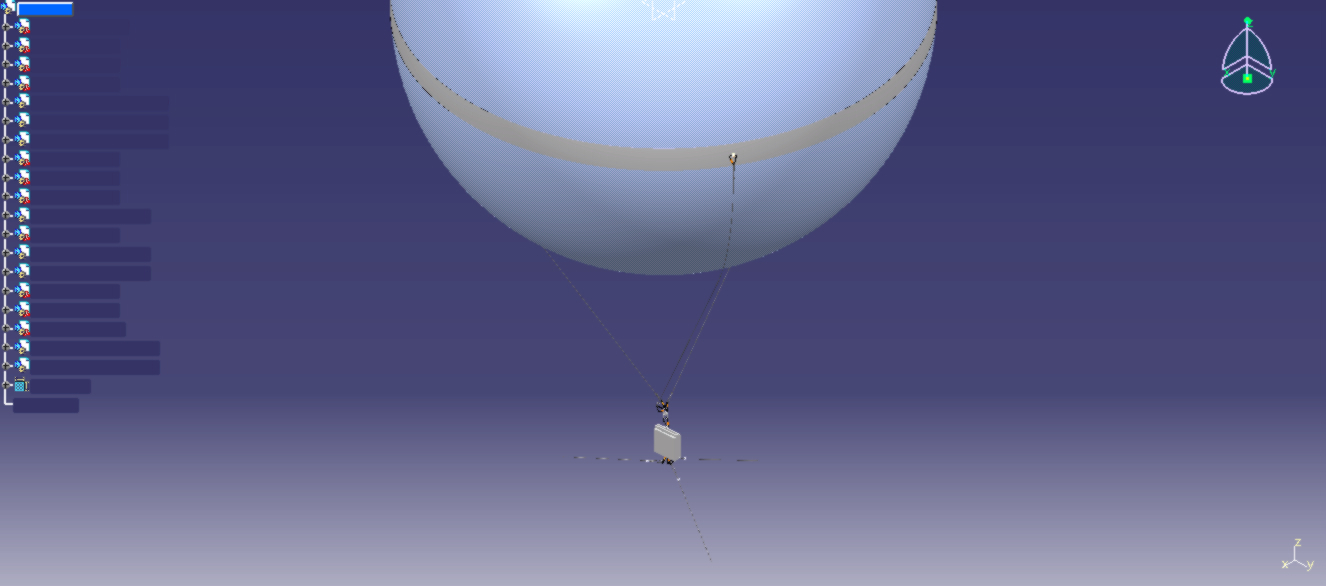
\includegraphics[width=0.6\textwidth]{figuras/catia1}
		\label{img:catia1}
	\end{figure}

	\begin{figure}[htp]
		\centering
		\caption{Protótipo da payload do SUM no Catia}
		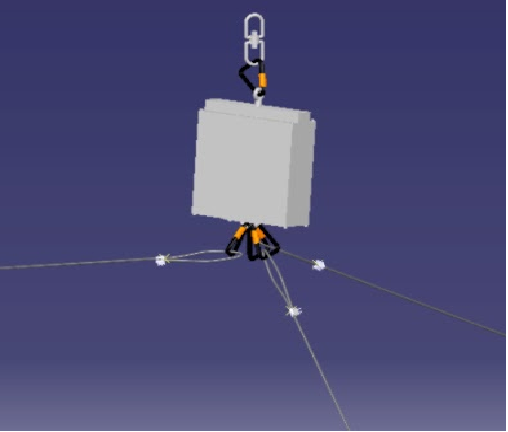
\includegraphics[width=0.6\textwidth]{figuras/catiadopayload}
		\label{img:catiaPayload}
	\end{figure}

	\begin{figure}[htp]
		\centering
		\caption{Detalhe do trilho da payload.}
		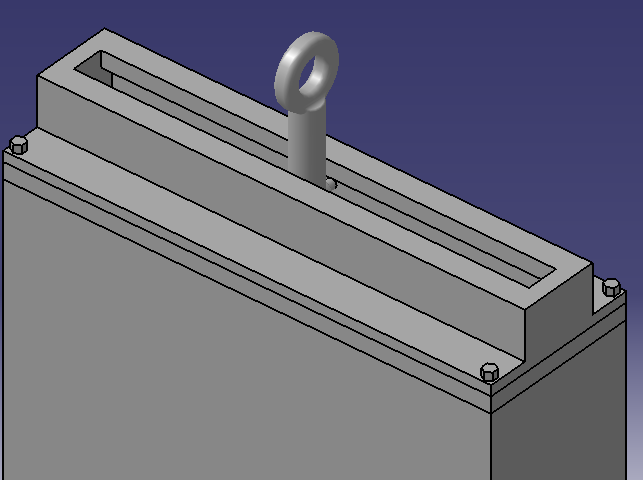
\includegraphics[width=0.6\textwidth]{figuras/catiadafixacao}
		\label{img:catia2}
	\end{figure}

A fixação será adaptada para cada um dos balões, pois como estarão em lugares distintos e estratégicos estudaremos cada um dos três pontos de fixação. A manutenção do balão será feita em solo, por exemplo: no caso de reposição do gás, na reparação de algum item interno da payload e etc. Para tal iremos utilizar dois motores elétricos para puxar o balão até o solo, os motores estarão fixos no chão onde será definido o local onde o cabo de sustentação será fixado, ou seja, o cabo de sustentação estará sendo regulado pelo motor.

De acordo com cálculos realizados previamente, a força resultante do balão será de aproximadamente de 6.4 KN. A partir destas informações, escolhemos o motor vendido pela empresa Bremen com a capacidade de 7240 Kg, potência de 4500W, 12V de tensão e pesando 52,5 Kg. A figura \ref{img:tabelamotor} mostra as informações referentes aos motores vendidos pela mesma empresa.

\begin{figure}[htp]
	\centering
	\caption[Tabela ilustrativa dos tipos de motores disponíveis]{Tabela ilustrativa dos tipos de motores disponíveis~\cite{bremem}}
	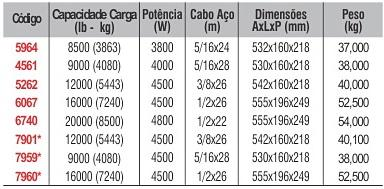
\includegraphics[width=0.8\textwidth]{figuras/tabelamotor}
	\label{img:tabelamotor}
\end{figure}

\begin{figure}[htp]
	\centering
	\caption[Modelo de motor elétrico escolhido]{Modelo de motor elétrico escolhido~\cite{bremem}}
	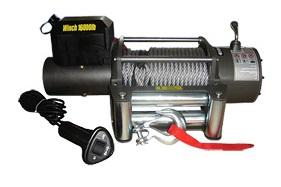
\includegraphics[width=0.8\textwidth]{figuras/modelodemotoreletrico}
	\label{img:motorescolhido}
\end{figure}

A figura \ref{img:motorescolhido} ilustra como será o motor. Para este motor será efetuada uma simples adaptação no cabo, onde será substituído o cabo de fábrica pelo cabo de aço classe 8x19 – Alma de Fibra com diâmetro de 6,4 mm. A alteração foi necessária em consideração ao peso do cabo, pois o mesmo é mais leve em relação ao cabo de aço comum, e também possui boas propriedades mecânicas como mostrado na figura \ref{img:motorescolhido}.

\begin{figure}[htp]
	\centering
	\caption[Propriedade do cabo Alma de Fibra]{Propriedade do cabo Alma de Fibra~\cite{acrocabo}}
	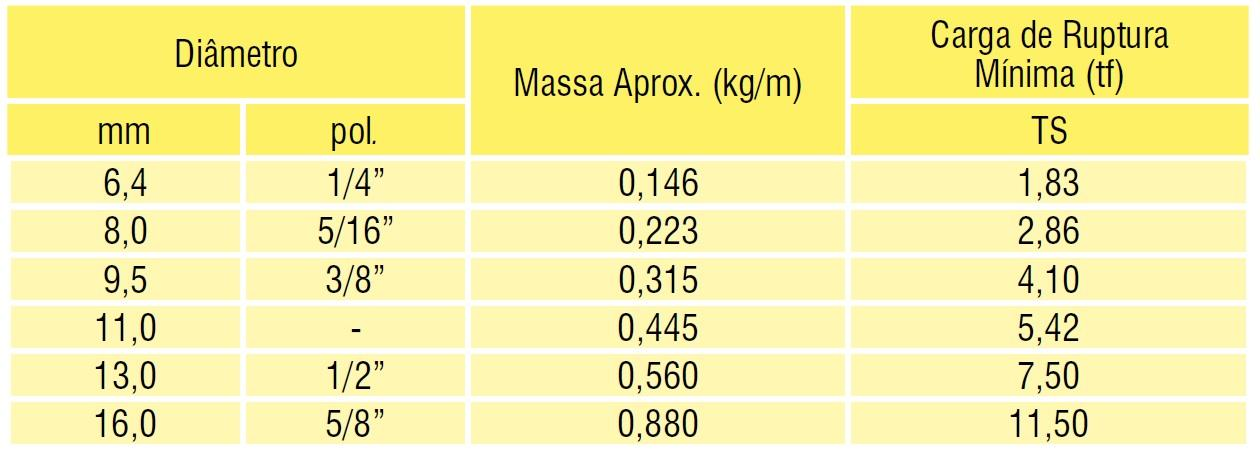
\includegraphics[width=0.8\textwidth]{figuras/tabelacabo}
	\label{img:motorescolhido}
\end{figure}

\subsection{Simulações na estrutura da payload}

	A estrutura interna da payload é dividida em duas superfícies e barras que conectam essas superfícies, como mostrado na figura \ref{img:payload3}.

	\begin{figure}[htp]
		\centering
		\caption{Estrutura interna da payload}
		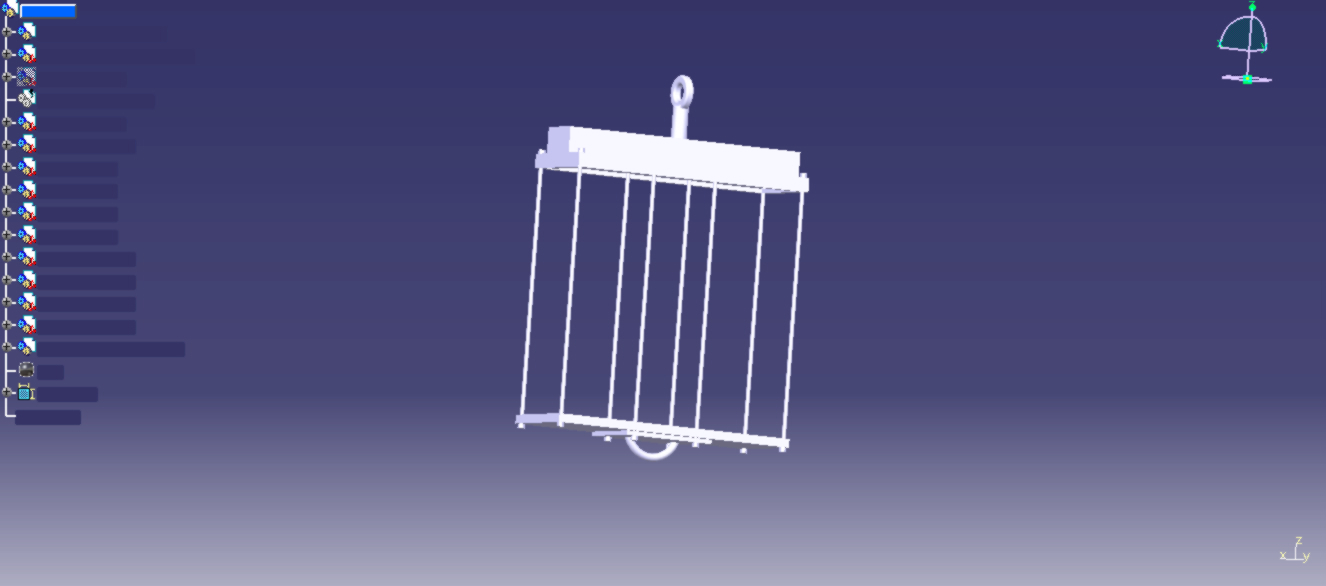
\includegraphics[width=0.8\textwidth]{figuras/payload3}
		\label{img:payload3}
	\end{figure}

	Deve-se analisar os pontos de maior deformação e concentração de tensão na estrutura da payload para que os equipamentos eletrônicos não sejam perdidos no meio da operação  do SUM. Simulações feitas no software CATIA V5R19 são agora analisadas.

	A figura \ref{img:maior-tensao} mostra onde a tensão está concentrada na payload, as barras de apoio entre as faces que “tampam” a payload também conectam os cabos ao envelope do balão, desta forma essas barras estão sempre tracionadas.

	\begin{figure}[htp]
		\centering
		\caption{Pontos de maior tensão na payload}
		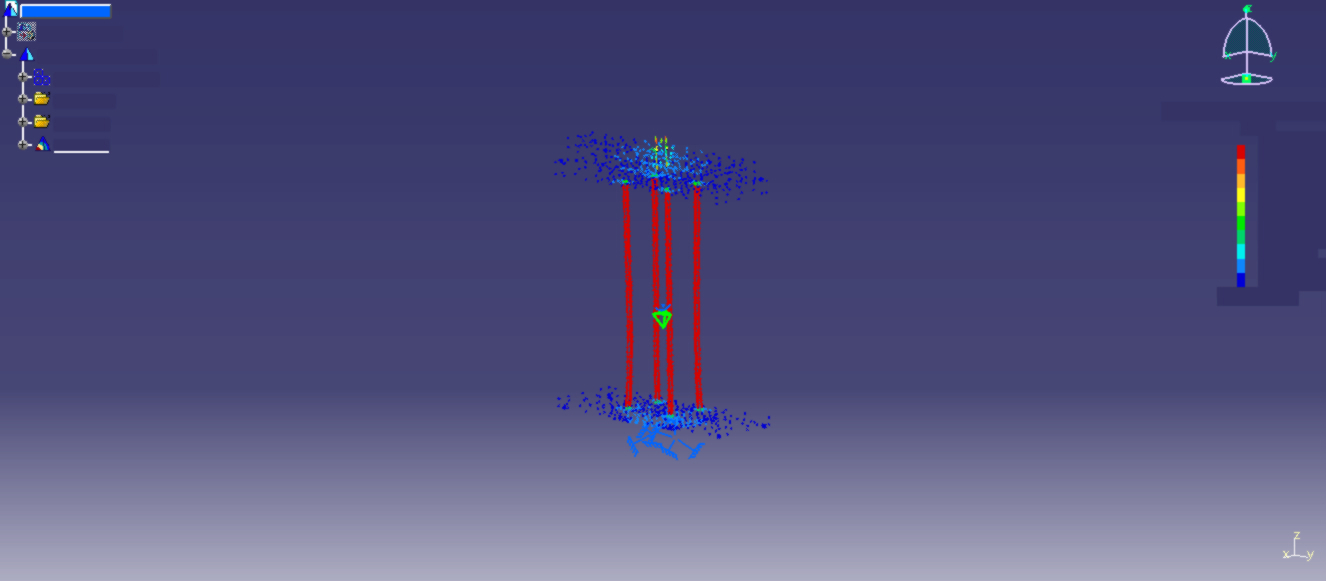
\includegraphics[width=0.8\textwidth]{figuras/maior-tensao}
		\label{img:maior-tensao}
	\end{figure}

	Os pontos passíveis de ocorrer deformação são mostrados na figura \ref{img:pontos-def}. A superfície em que o envelope é conectado à payload poderá sofrer maior, enquanto que as barras que sofrem tração na figura \ref{img:maior-tensao} podem se romper próximos a essa superfície.

	\begin{figure}[htp]
		\centering
		\caption{Pontos de possível deformação}
		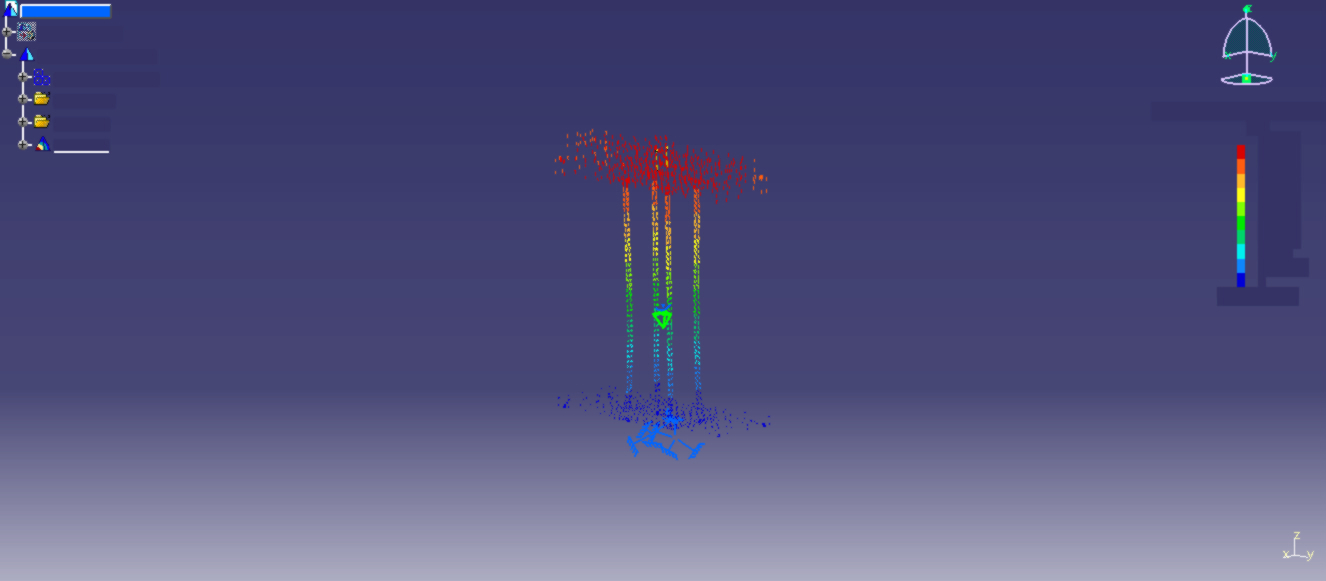
\includegraphics[width=0.8\textwidth]{figuras/pontos-def}
		\label{img:pontos-def}
	\end{figure}

	Portanto, durante as manutenções deve-se verificar se essas áreas ainda estão aptas para o desempenho de suas funções.


\subsection{Mudanças no projeto do balão}

O cronograma previsto para o ponto de controle 3 previa apenas alguns ajustes pontuais na escolha dos materiais e a pesquisa de preço, porém houve um aspecto na apresentação que foi questionado pelos avaliadores com relação a vazão em massa do gás, as suposições feitas para esse cálculo estariam equivocadas. Para solucionar esse problema, foi proposto a utilização de sensores para medir o empuxo líquido do balão, porém para empregar esses sensores teríamos de calibra-los para saber o comportamento do balão.

O que foi discutido entre o subgurpo de estrutura do balão foi a questão de não haver tempo viável para a pesquisa desses sensores e a calibração dos mesmos, sem contar que  as adaptações no projeto poderiam levar a mudança de alguns materiais já pesquisados, e consequentemente, as contas referentes a sustentação do balão no solo também sofreriam modificações. Visando diminuir o impacto dessas mudanças no projeto, foi proposto por membros do grupo que mudássemos o sistema do balão de Zero Pressão para Super Pressão, sem que houvesse mudança na massa total do sistema para não alterar toda a cadeia de cálculos. As próximas seções apresentam como chegamos a conclusão de que a mudança de sistema é viável para o projeto.

A pesquisa de mercado também não encontrou os materiais para o envelope do balão ideais, desta forma houve uma mudança no material do balão do ponto de controle 2 para o ponto de controle 3. Esse tópico será melhor abordado nas próximas seções.

\subsubsection{Novo dimensionamento do balão}

Os cálculos anteriores chegaram aos seguintes valores:
\begin{itemize}
	\item Volume do balão: 113,1 $m^3$
	\item Massa de hélio: 17 kg
\end{itemize}

A mudança desses dois valores acarretaria na mudança da maioria dos cálculos já realizados, especialmente o volume do balão, que afeta a força de empuxo. A mudança no valor da massa de hélio não é um fator tão importante quanto o volume, pois a massa de hélio é pequena se comparada com o resto da estrutura.

Considerando que o PVC pneumático possui resistência a tração de 40 Mpa, o Polietileno Linear de baixa densidade (PELBD) possui uma resistência à tração de 37 MPa, o Polietileno de baixa densidade (PEBD) possui resistência à tração de 24 MPa, e adotando um fator de segurança de 150, pois qualquer dos materiais escolhidos vão trabalhar em condições adversas de temperatura, chega-se a conclusão de que a pressão interna do balão não deve ultrapassar 240 kPa (1.6 atm). Portanto, adotou-se o valor de 1.5 atm como a pressão máxima permitida para o balão.

Usando a equação dos gases ideias,considerando o hélio como um gás ideal e admitindo uma temperatura de 39$^{\circ}$ (312.15 K), que é uma das temperaturas mais altas registradas na cidade do Gama,  pode-se calcular a massa de hélio para sabermos um valor de referência.

\begin{equation}
	PV = nRT \Rightarrow n =  \frac{113100\cdot1.5}{0.082\cdot312.15} \Rightarrow n = 6.63\cdot10^3 mols
	\label{gasideal}
\end{equation}

onde:

\begin{itemize}
	\item \textbf{P} é a pressão,
	\item \textbf{V} é o volume,
	\item \textbf{n} é o número de mols,
	\item \textbf{R} é a constante universal dos gases (0.082 $atm\cdot l/mol\cdot K$), e
	\item \textbf{T} é a temperatura.
\end{itemize}

Como a massa total é o número de mols multiplicado pela massa molar, chega-se ao valor de 26.5 kg de hélio.

Como a alteração do valor da massa do hélio não é muito grande não haverá mudanças com relação ao sistema de sustentação balão.

\subsubsection{O material}

O Balão \textit{Super-Pressão} funciona de tal forma que começará a descender quando sua pressão interna diminuir a um nível menor que a pressão externa. Um balão perde gás naturalmente em decorrência da passagem de moléculas do gás pelo material do envelope. Escolhemos o material do balão como sendo PVC pneumático que apresenta uma permeabilidade de  5$cm^3/ml\cdot24h\cdot atm$   valor que relaciona o volume de  perda do material pelo volume que ele suporta e a pressão em seu interior a cada 24h.

Temos um balão de volume 113.1$m^3$ que suporta uma pressão de 1.5 atm, isso nos dá uma perda de 0.3 atm por dia.

Temos que determinar o tempo que leva para a pressão no interior do balão atingir 1 atm considerando que seu volume permanece constante. Utilizando a equação geral dos gases perfeitos, equação \label{gasideal}, temos que a variação de pressão no balão considerando uma variação de 0,3$m^3$ por dia é de $3.87\cdot10^{-3}$ atm/dia.

A quantidade de dias necessários para se perder 0.5 atm e atingir o nível onde o balão começa a descer é de aproximadamente 129 dias, o que nos da um perda total de 38.7$m^3$ de gás. Ressalta-se que o volume do balão permanece inalterado desde que a pressão interna do balão seja maior que a pressão externa, desta forma o empuxo líquido não varia se a manutenção for feita no período estipulado.

A massa específica do PVC é de 1390$kg/m^3$, o envelope balão terá uma área superficial de 113$m^2$ e uma espessura de 0.23 mm. Desta forma a massa total desse material será de aproximadamente de 36.2 kg.


\subsection{Peso total da estrutura}
Com as mudanças no material e na quantidade de gás o peso total da estrutura também será alterado. As alterações são mostradas na tabela \ref{tab:forcanova}.

\begin{table}[htp]
	\centering
	\caption{Alteração nas forças atuantes na estrutura}
	\begin{tabular}{ | c || c | c |}
		\hline
		\textbf{Força} &\textbf{Anterior} &\textbf{Atual} \\ \hline
		\textbf{Empuxo} & 1232.1 N & 1232.1 N \\ \hline
		\textbf{Peso do Hélio}  & 170 N& 260.7 N \\\hline
		\textbf{Peso do envelope} & 62.5 N&  354.4 N\\ \hline
		\textbf{Peso dos cabos} & 100 N &  100 N \\\hline
		\textbf{Peso Extra} & 20 N &  20 N \\\hline
		\textbf{Peso da \textit{Payload}} & 100 N &  100 N \\\hline
		\textbf{Empuxo Líquido} & 780 N &  397 N \\
		 \hline
	\end{tabular}
	\label{tab:forcanova}
\end{table}

O peso dos cabos, da payload e outros componentes não sofreram alteração. Com a tabela \ref{tab:forcanova} percebe-se que a maior mudança foi no empuxo líquido, mas essa alteração não influencia nos cálculos feitos para o esforço nos cabos, visto que eles já conseguiam sustentar a estrutura antes da alteração.

\subsection{Preços}

\hspace{1cm}

\begin{enumerate}

	\item \textbf{POSTE}

		As empresas POSTEFER, REPUME iluminações e TROPICO foram procuradas para solicitação de orçamento do poste para fixação do cabo. Somente a empresa REPUME respondeu a solicitação. Os produtos são os seguintes:

		\begin{itemize}
			\item Poste Cônico Contínuo Reto Flangeado, fabricado em chapa de aço SAE 1010/1020. Com 10 metros de altura útil. Diâmetro de base 170 mm, diâmetro de topo 60,3 mm.
			\item Chumbador para a fixação de flange do poste 3/4" X 500 X 70 mm com porcas e arruelas.
		\end{itemize}

		Os preços são mostrados na tabela \ref{tab:precoposte}. São 4 postes de fixação de apoio para o balão e 16 pontos de fixação.

		\begin{table}[htp]
			\centering
			\caption{Preços do poste (Fixação)}
			\begin{tabular}{ | c | c | c | c |}
				\hline
				\textbf{Qdt} &\textbf{Peça} &\textbf{Preço unitário} &\textbf{Preço total}\\ \hline
				4 & Poste & R\$ 1.389,00 & R\$ 5.556,36 \\ \hline
				16 & Chumbador & R\$ 21,41 & R\$ 342,56 \\
				 \hline
			\end{tabular}
			\label{tab:precoposte}
		\end{table}

		Em relação aos cabos de fixação, serão necessários 100 metros do cabo de aço classe 8x19 alma de Fibra com diâmetro de 6.4 mm, como já foi apresentado. As empresas  A.CAMARGO, CABLEMAX,  SIVA forneçem o produto, o preço médio do metro é de  R\$ 5,00, portanto o preço total é R\$ 480,00.

		\hspace{1cm}

	\item \textbf{MOTOR}

		A tabela \ref{tab:precomotor} mostra a quantidade de cada material que cada balão vai precisar para ser fixado no teto do prédio.

		\begin{table}[htp]
			\centering
			\caption{Preços do restante dos materiais da sustentação (Fixação)}
			\begin{tabular}{ | c | c |}
				\hline
				\textbf{Quantidade} &\textbf{Item} \\ \hline
				1 &Guincho Winch 8500 lbs / 3.850Kg com cabo de aço com 28 metros \\ \hline
				1 &Controle remoto com cabo de 3 metros \\ \hline
				1 &Gancho\\ \hline
				1 &Rolete guia\\ \hline
				1 &Caixa de solenoide\\
				 \hline
			\end{tabular}
			\label{tab:precomotor}
		\end{table}

		O modelo do guincho é o seguinte: Guincho Winch 8.500lbs / 3.850Kg, linha profissional com cabo de aço com 28 metros c/ Controle remoto COM FIO + Gancho+ Rolete guia + Caixa de solenoide.

		Custo Unitário dos itens da tabela \ref{precomotor} excetuando o guincho : R\$1876,00 + R\$ 118,92 = R\$1994,92. Os R\$ 118,92 são referentes ao frete que tem o prazo de 5 dias. Como serão necessários mais de um motor para cada balão, caso a compra seja no atacado cada um é vendido a R\$1700,00. Cada balão precisará de 2 conjuntos dos itens da tabela \ref{precomotor}. O custo total para os 5 balões é de R\$36.949,20. Os preços foram obtidos a partir de pesquisa e comparação entre concorrentes, escolhendo a empresa \cite{precoMotor}.

		\hspace{2cm}
	\item  \textbf{GÁS HÉLIO}

		Dentre as distribuidoras de gás hélio no Distrito Federal analisamos a concorrência entre a Oxigmed Gases e Equipamentos e a Praxair. Optamos por utilizar cilindros de 10$m^3$ de hélio para inflarmos o balão. A tabela \ref{precogas} mostra o preço do gás em duas fornecedoras.

		\begin{table}[htp]
			\centering
			\caption{Preço do gás Hélio}
			\begin{tabular}{ | c | c | c |}
				\hline
				\textbf{Fornecedor} &\textbf{Preço unitário do cilíndro} &\textbf{Preço total}\\ \hline
				Oxigmed Gases e Equipamentos & R\$ 1.650,00 & R\$ 19.800,00 \\ \hline
				Praxair & R\$ 1.330,00 & R\$ 15.960,00 \\
				 \hline
			\end{tabular}
			\label{precogas}
		\end{table}

		Como o balão tem um volume de 113,1 $m^3$ serão necessários aproximadamente 12 cilindros para inflar o balão.

		Optamos pela distribuidora Praxair como fornecedora de gás hélio em decorrência do menor preço e confiabilidade. Como teremos um total de 5 balões será necessário um valor de R\$ 79.800,00.

		A empresa Park e Ação faz a recarga de cilindros vazios. O preço para recarregar 2$m^3$ de hélio é de R\$ 200,00.

		Considerando o preço do volume de gás hélio como R\$ 100,00 o metro cúbico e arredondado o valor da reposição para 40$m^3$ de gás por balão será necessário repor 200$m^3$ por R\$100,00 o metro cúbico de gás ao final de 4 meses. O que nos dá um valor de R\$ 20.000,00 a cada 4 meses. Desta forma, o gás do balão terá um custo médio mensal de R\$5.000,00.

		\begin{itemize}
			\item Custo inicial do gás: R\$  79.800,00
			\item Custo mensal do gás:  R\$5.000,00.
		\end{itemize}

		Estes valores foram obtidos atraves de pesquisa e seleção de fornecedor, escolhendo as empresas \cite{precoGasHelio} e \cite{oxigmed}.

		\hspace{1cm}

	\item  \textbf{Material do envelope}

		A pesquisa apontou que dois materiais poderiam ser usados para o confeccionar o envelope do balão, o polietileno linear de baixa densidade (PELBD) e o polietileno de baixa densidade (PEBD), porém na pesquisa de mercado não foi encontrado uma empresa que fornecessem e/ou confeccionassem o envelope.

		Uma saída para a solução desse imprevisto foi a comprar de balões inflãveis do tipo Blimp como mostrado na figura \ref{img:blimp2}, esses balões são feitos com PVC pneumático.

		\begin{figure}[htp]
			\centering
			\caption{Exemplo de balão \textit{blimp} usado em publicidade. Fonte: OLX}
			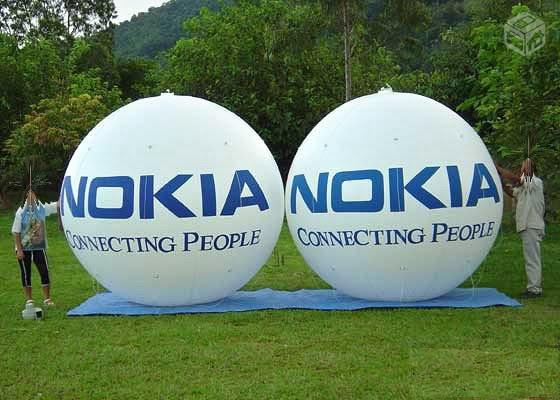
\includegraphics[width=8cm, height=5cm]{figuras/blimp}
			\label{img:blimp2}
		\end{figure}

		O preço desse tipo de balão é por volta de R\$ 1000,00, dependendo do tamanho do balão. A empresa Fly Balloon foi solicitada via-email para o orçamento de um balão Blimp esférico de 3 metros de raio. As informações constam na tabela \ref{tab:precoblimp}.

		\begin{table}[htp]
			\centering
			\caption{Informações sobre o balão}
			\begin{tabular}{ | c | c |}
				\hline
				\textbf{Característica} &\textbf{Valor numérico} \\ \hline
				Raio & 3 metros  \\ \hline
				Material  & PVC pneumático \\
				 \hline
				Preço  & R\$ 1.100,00 \\
				 \hline
			\end{tabular}
			\label{tab:precoblimp}
		\end{table}

		Como serão 5 balões, o valor total será de  R\$ 5.500,00. Este valores foram obtidos a partir de pesquisa na empresa \cite{balloon}.
\end{enumerate}

\subsubsection{Custo total da estrutura}

	Após realização de pesquisa e seleção de fornecedores, todos os valores foram compilados, chegando ao seguinte resultado:

\begin{itemize}
	\item Custo inicial total: R\$ 128.628,02
	\item Custo mensal total: R\$ 5.000,00
\end{itemize}
